\documentclass[12pt]{article}

	\usepackage{graphicx}
	\usepackage[round]{natbib}

	\linespread{1.3}
	\bibliographystyle{plainnat}

	\title{
		Group \#07 \\
		Bridge-00 \\
		18g, 1700N \\[1cm]
		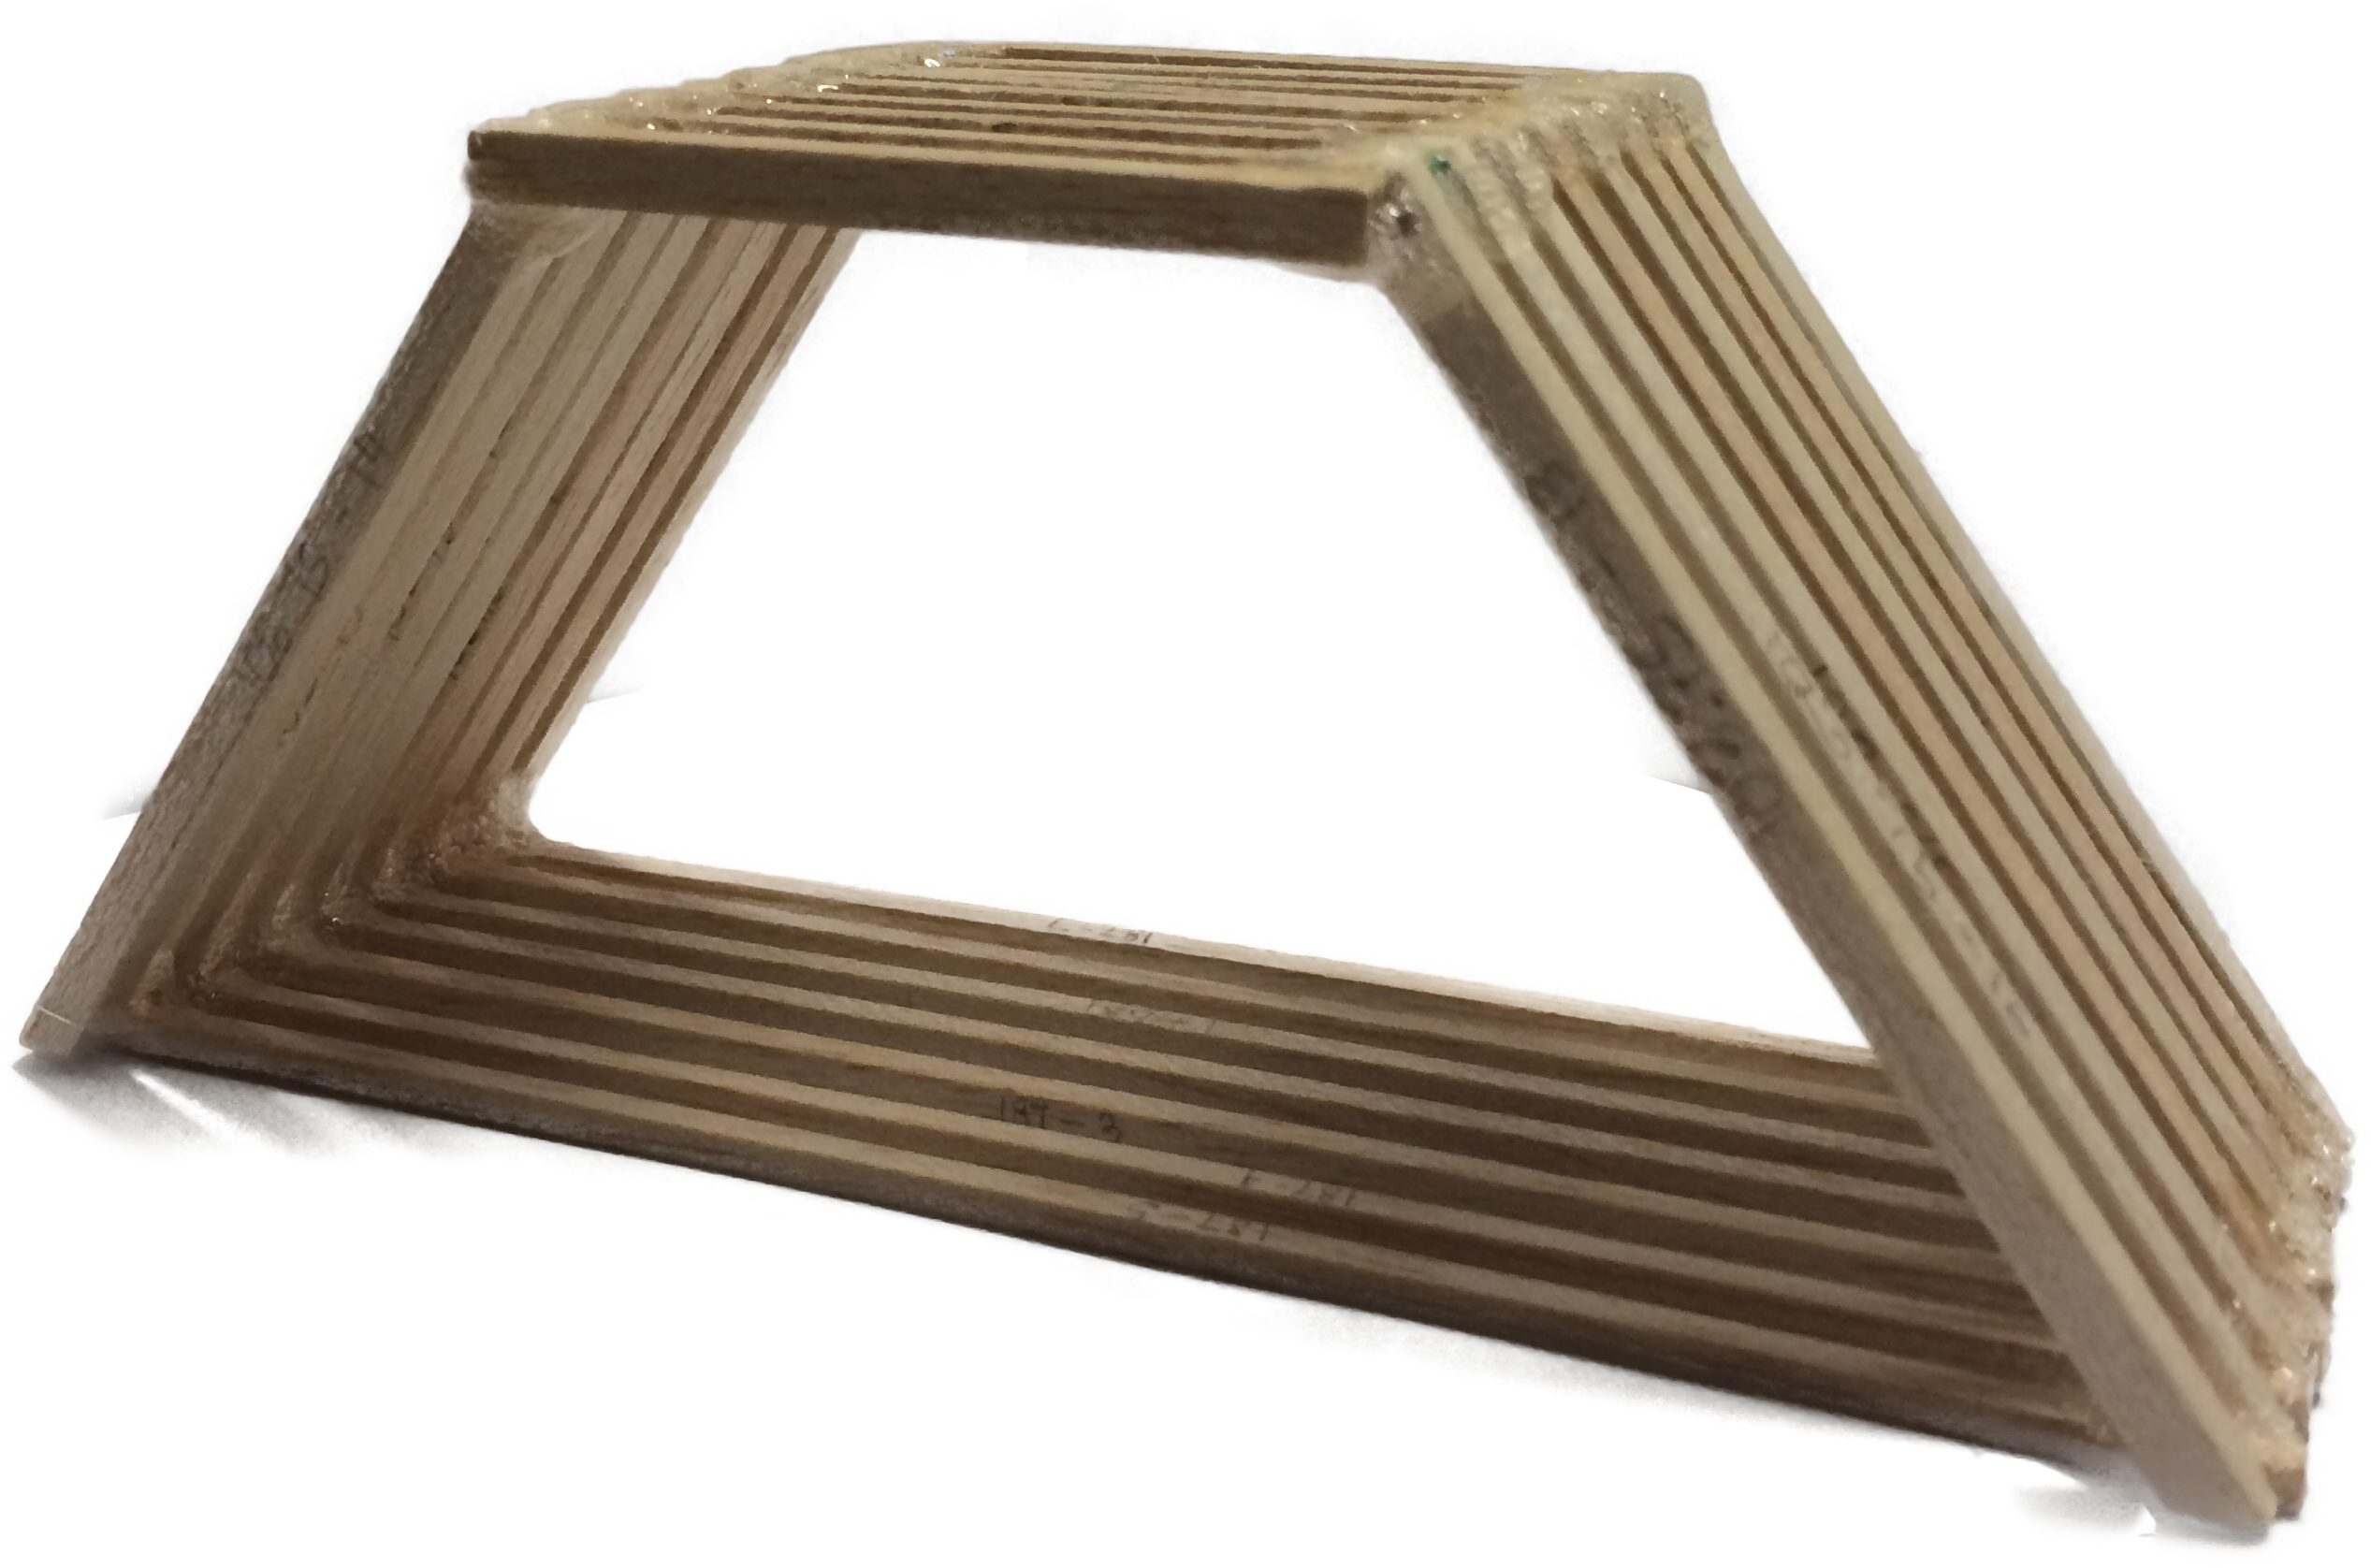
\includegraphics[width=0.7\textwidth]{photo}
	}

	\author{
		Alex Miles \\ u5568175 \\ 16.7\%
		\and Arlene Mendoza \\ u5589650 \\ 16.7\%
		\and Itsuki Nishida \\ u5578430 \\ 16.7\%
		\and Paul Apelt \\ u5568225 \\ 16.7\%
		\and Stephen Lonergan \\ u5349877 \\ 16.7\%
		\and Thomas Hale \\ u5568225 \\ 16.7\%
	}

\begin{document}
	\maketitle

	\section{Design}

		% design assumptions and methods

		\subsection{Assumptions}
		During the design process, the following assumptions have been made \citep[p.~264]{tbook}:

		\begin{enumerate}
			\item All loadings are applied at the joint,
			\item Weight of the members neglected,
			\item Joints are smooth (friction-less) pins,
			\item Each member has no more than two joints.
		\end{enumerate}

		% TODO: why trapezium
		% other designs considered
		% photo of a prototype

		Final bridge design can be seen in Figures \ref{dim} and \ref{proj}.

		\begin{figure}[h!]
			\centering
			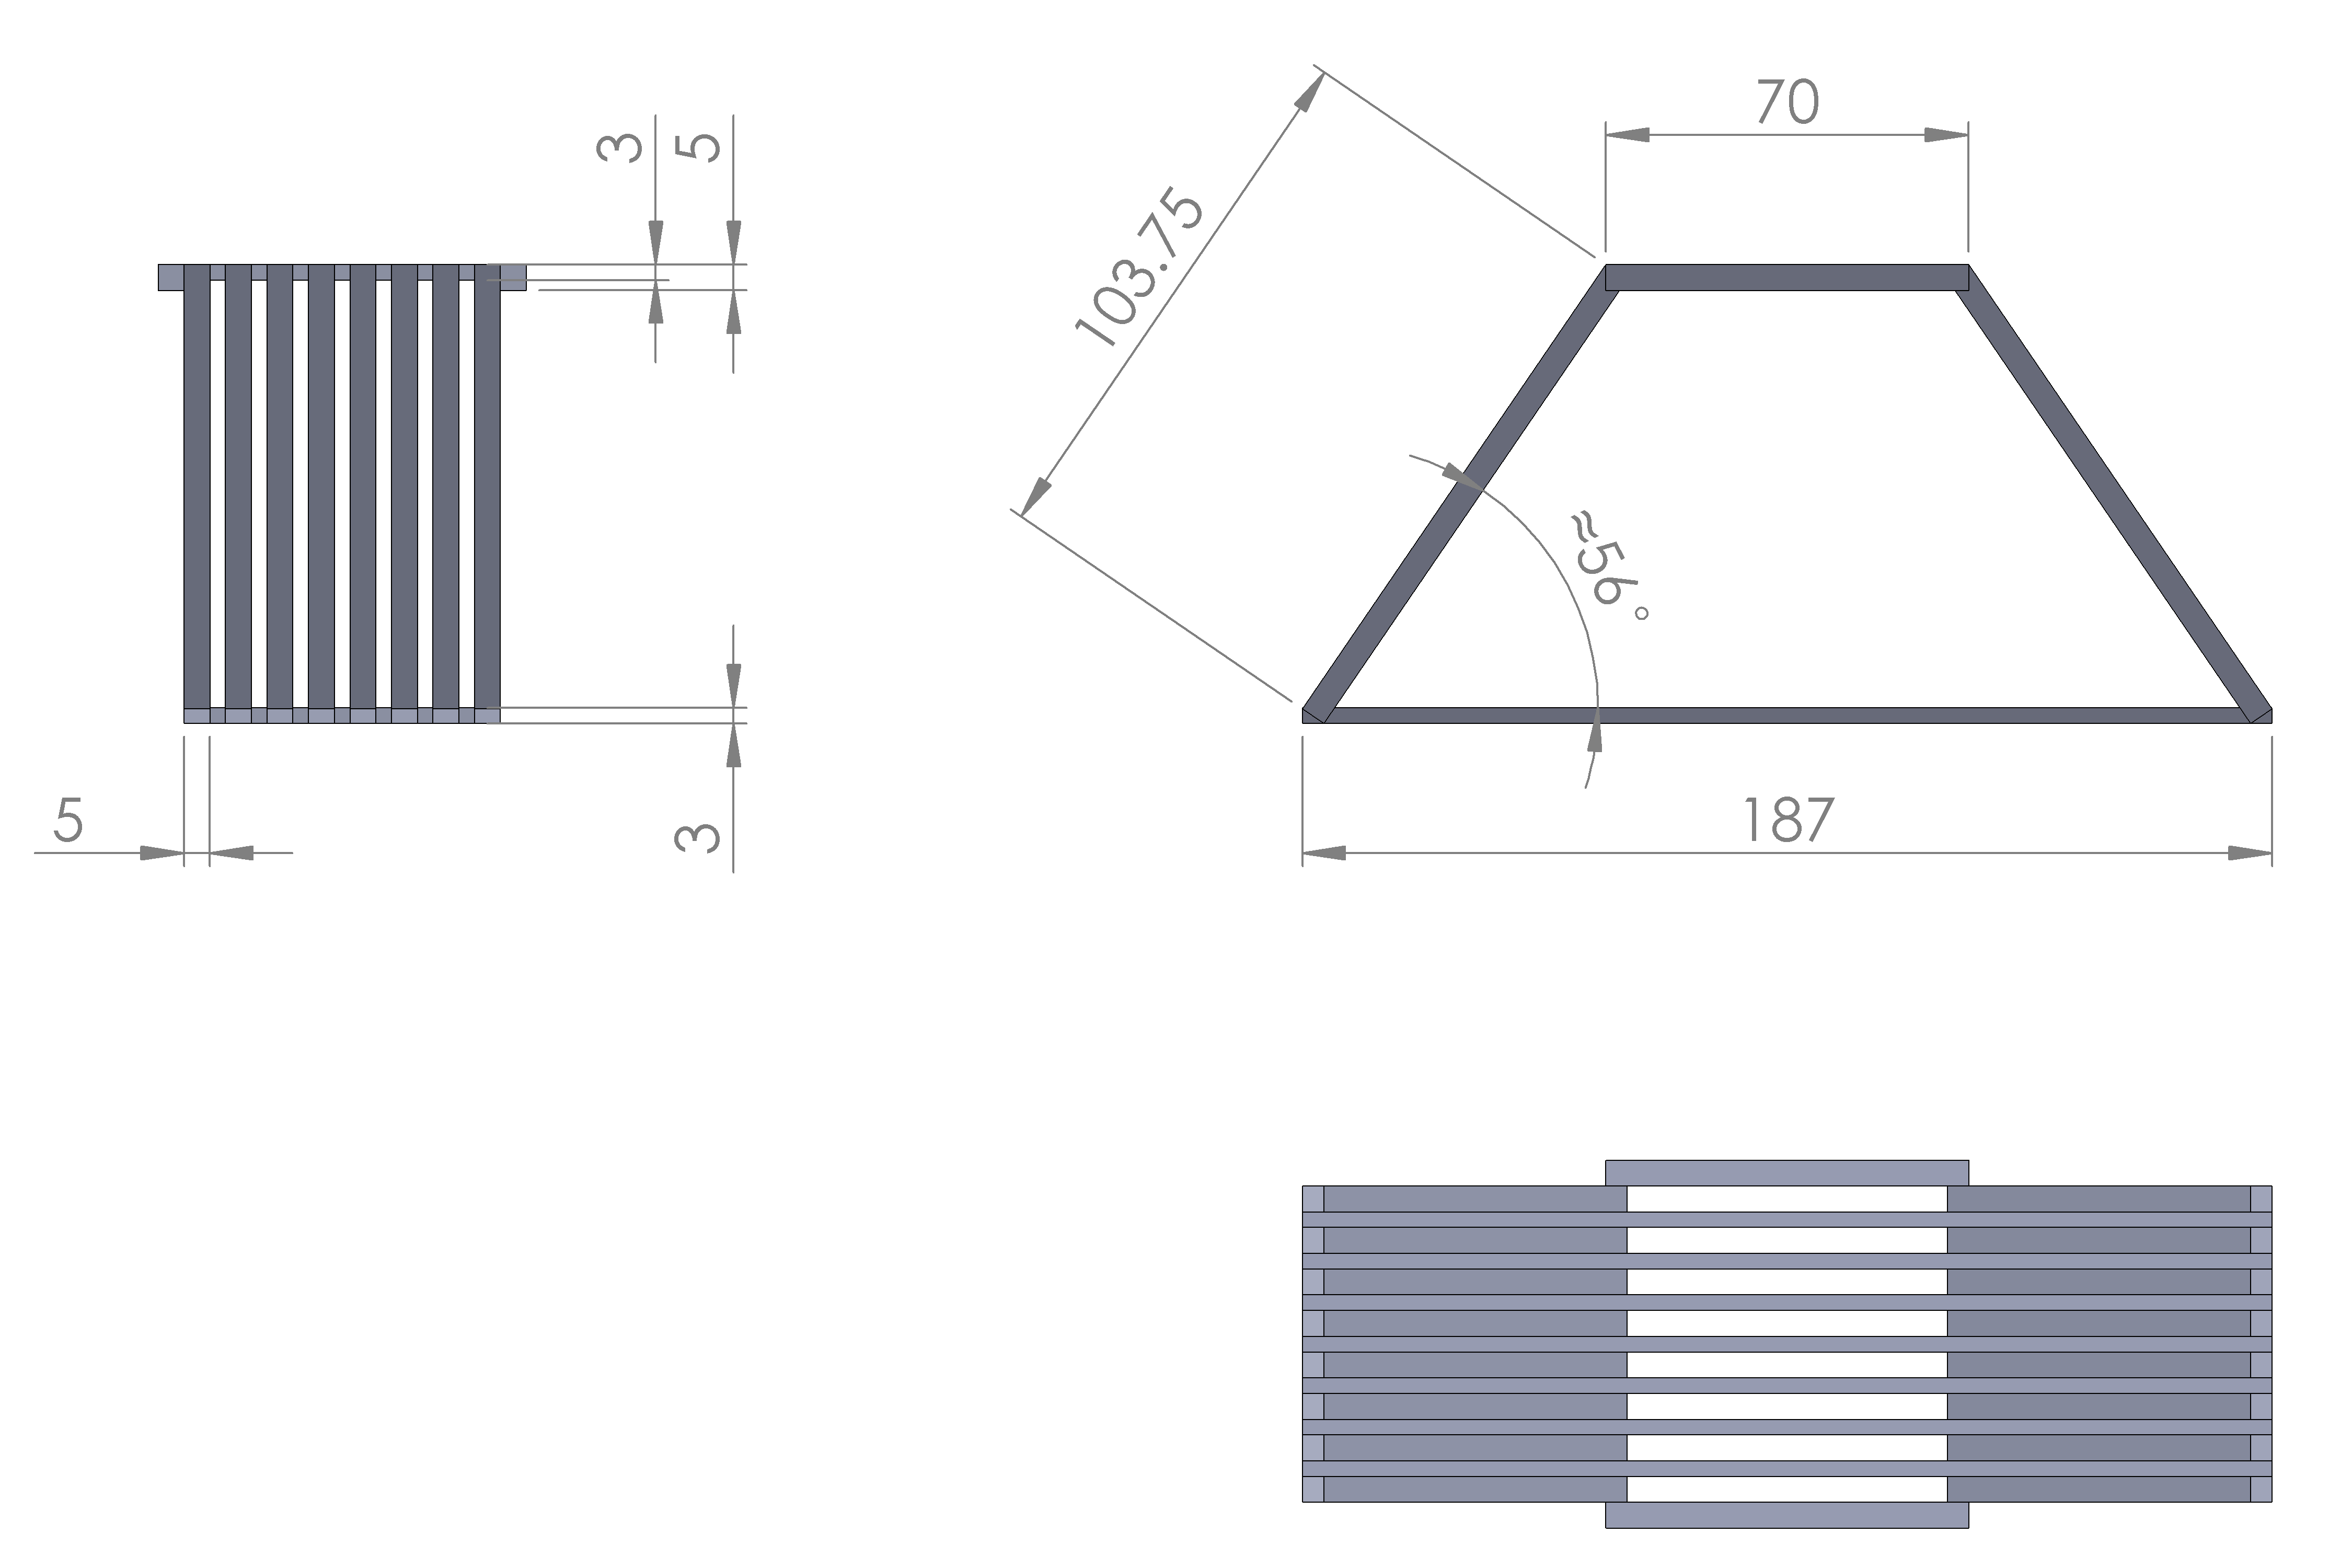
\includegraphics[width=\textwidth]{dim}
			\caption{Dimensioned drawing.}
			\label{dim}
		\end{figure}

		\begin{figure}[h!]
			\centering
			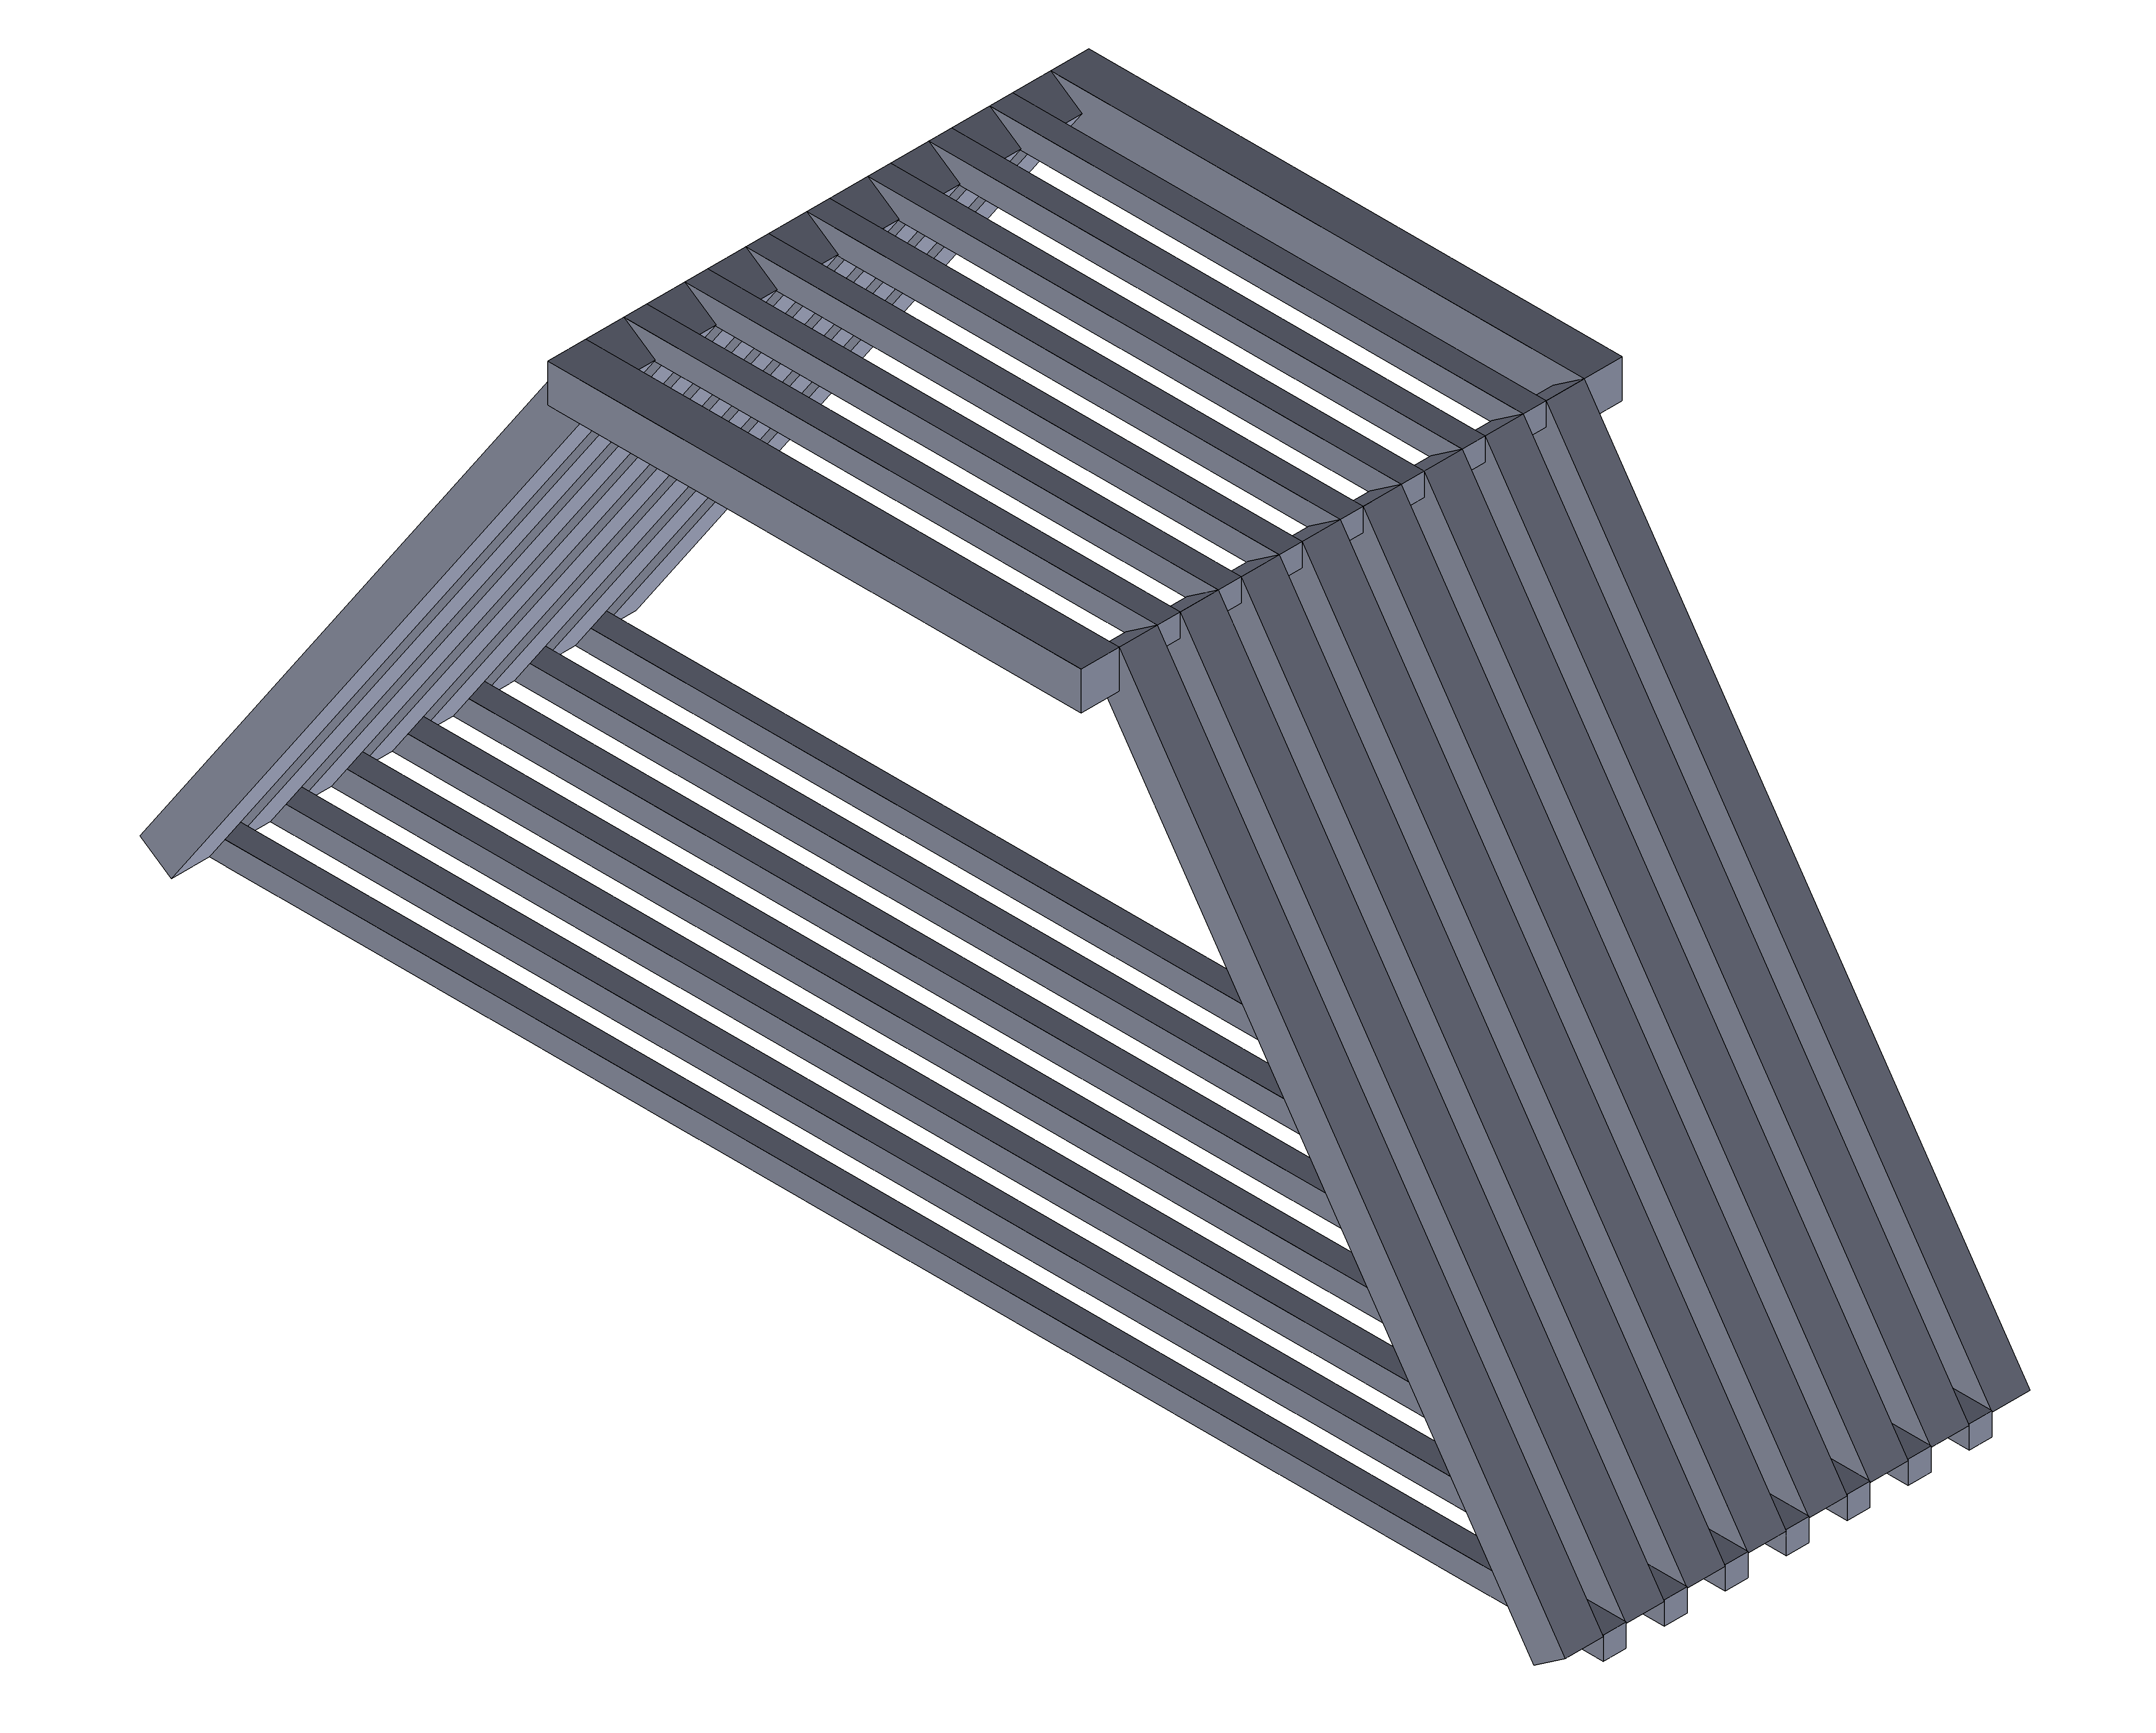
\includegraphics[width=0.6\textwidth]{proj}
			\caption{3D-Projection.}
			\label{proj}
		\end{figure}

		% dimensioned drawing

		\subsection{Methods}

		% construction process 
		% materials Used
		% difficulties faced - measuring accurately, It ended up being 185mm than 187mm and the trapezium was also slightly lopsided by a 1mm
		% weight issues - excess glue fail 
		% picture of the materials used

	\section{Analysis}

		Due to the unconventional design, to ease the calculations during the analysis, it was assumed that the load is equally distributed between eight trapezium-shaped trusses. Thus, a single trapezium truss was analyzed, and then extended to approximate the entire bridge.

		% insret calculations here

		The table of forces in each member of the trapezium truss under a load of 100N across the top two nodes can be seen in Table~\ref{loads}.
		
		% table of member loads

		\begin{table}[h!]
			\caption{Member loads}
			\begin{center}
			\begin{tabular}{ | r | l | }
				\hline
				70 3x3 mm (top) & 34.14 N (c) \\ \hline
				103.75 5x5 mm (side) & 60.54 N (c) \\ \hline
				187 3x3 mm (bottom) & 34.14 N (t) \\ \hline
			\end{tabular}
			\end{center}
			\label{loads}
		\end{table}

		% assumptions
		% fail predictions
		% max load
		% reasons

	\section{Results}

		% analysis of the difference
		% why fail
		% much sad
		% testing machine OP
		% please nerf
		%Add pic of the final bridge and show the glue
		%What was the final load it could hold?

	\bibliography{bib}
\end{document}

